\documentclass{article}
\usepackage{amsmath}
\usepackage{graphicx}
\usepackage{geometry}
\usepackage{caption}
\usepackage{tikz}
\usepackage{float}
\usepackage{hyperref}
\usepackage{minted}
\usepackage[backend=biber, style=authoryear]{biblatex}

\geometry{margin=1in}

\title{Understanding the U-Net Architecture with Code}
\author{}
\date{}

\addbibresource{references.bib}

\begin{document}

\maketitle

The U-Net is made up of contracting path (downsampling), bottleneck (middle part) and expansive path (upsampling).

\begin{figure}[H]
    \centering
    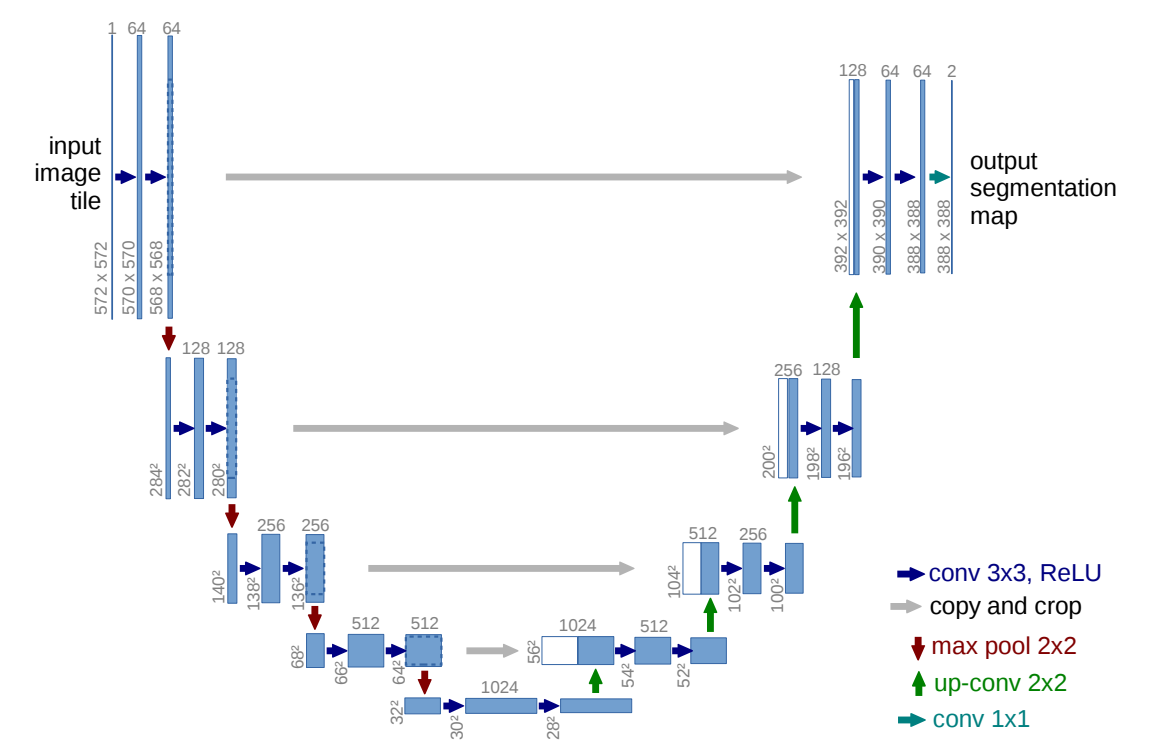
\includegraphics[width=0.8\textwidth]{unet.png}
    \caption{U-Net Architecture}
    \label{fig:unet}
\end{figure}

\tableofcontents
\newpage

\section{Contracting Path (Downsampling)}

The contracting path captures the context of the input image by applying repeated convolution and pooling operations. Each step in the contracting path contains:

\begin{itemize}
    \item \textbf{\textcolor{blue}{Blue arrow}}: Two $3 \times 3$ convolutional layers (with ReLU activation after each convolution layer).
    \item \textbf{\textcolor{red}{Red arrow}}: A $2 \times 2$ max pooling layer with stride 2 for downsampling.
\end{itemize}





\subsection{Blue arrow: Convolutional block}

\begin{figure}[H]
    \centering
    \begin{tikzpicture}
        \node[anchor=south west, inner sep=0] (img) at (0,0) {
            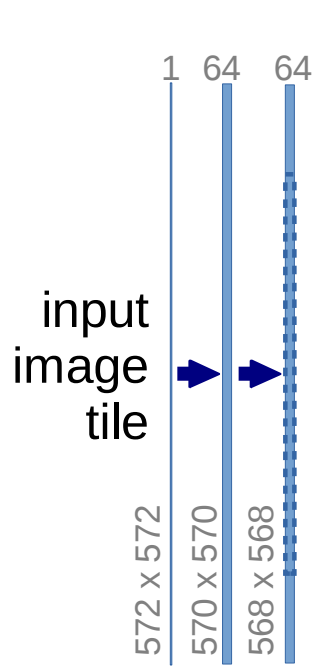
\includegraphics[width=0.15\textwidth]{latex/blue_arrow.png}
        };

        \begin{scope}[x={(img.south east)}, y={(img.north west)}]
            \draw[red, thick] (0.55,0.0) rectangle (0.75, 0.95);
            \node[text opacity=1, text=red] at (0.55, 1.0) {Conv 1 + ReLU};

            \draw[blue, thick] (0.75,0.0) rectangle (0.95, 0.95);
            \node[text opacity=1, text=blue] at (0.95, -0.05) {Conv 2 + ReLU};

            \draw[black, thick] (0.0,-0.01) rectangle (1.0, 0.96);
            \node[text opacity=1.0] at (1.6, 0.5) {DoubleConvolution};
        \end{scope}
    \end{tikzpicture}
    \caption{Double Convolutional Block}
\end{figure}

The double convolution block can be defined as:

\begin{minted}[fontsize=\small, linenos]{python}
class DoubleConvolution(nn.Module):
    def __init__(self, in_channels, out_channels):
        super().__init__()
        self.conv_block = nn.Sequential(
            nn.Conv2d(in_channels, out_channels, kernel_size=3, padding=1),
            nn.ReLU(inplace=True),
            nn.Conv2d(out_channels, out_channels, kernel_size=3, padding=1),
            nn.ReLU(inplace=True)
        )
    
    def forward(self, x):
        return self.conv_block(x)
\end{minted}

Explanation of the code:

\begin{itemize}
    \item The padding of 1 ensures that the spatial dimensions remain the same after convolution. Though in the original paper \cite{unet}, there was no padding; we can see this in figure \ref{fig:unet} where we go from $572 \times 572$ to $570 \times 570$ by the first convolution with kernel size $3 \times 3$, which makes sense.
    
    \item The \texttt{inplace=True} argument in ReLU allows for memory optimization by modifying the input directly (instead of allocating memory).
\end{itemize}









\subsection{Red arrow: Maxpooling}

\begin{figure}[H]
    \centering
    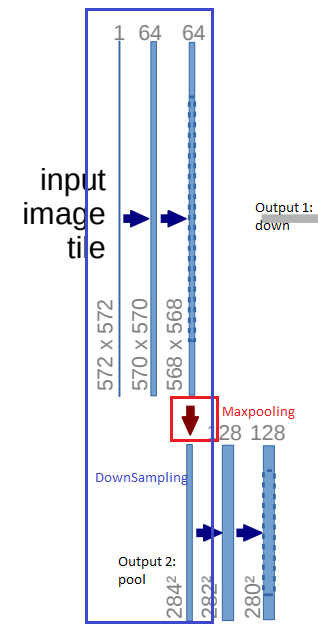
\includegraphics[width=0.25\textwidth]{latex/red_arrow.png}
    \caption{Downsampling Block}
    \label{fig:downsamlping_block}
\end{figure}

The downsampling operation can be implemented as:

\begin{minted}[fontsize=\small, linenos]{python}
class DownSampling(nn.Module):
    def __init__(self, in_channels, out_channels):
        super().__init__()
        self.conv = DoubleConvolution(in_channels, out_channels)
        self.pool = nn.MaxPool2d(kernel_size=2, stride=2)
    
    def forward(self, x):
        down = self.conv(x)
        pool = self.pool(down)

        return down, pool
\end{minted}

Explanation of the code:

\begin{itemize}
    \item We apply a single \texttt{DoubleConvolution} block to the input, and then we apply the maxpooling operation on the result, which is shown in figure \ref{fig:downsamlping_block}.
    \item We return both the output of the \texttt{DoubleConvolution} block which will be used for the skip connection and the output of the maxpooling operation which will be used for the next downsampling block.
\end{itemize}













\section{Bottleneck}

\begin{figure}[H]
    \centering
    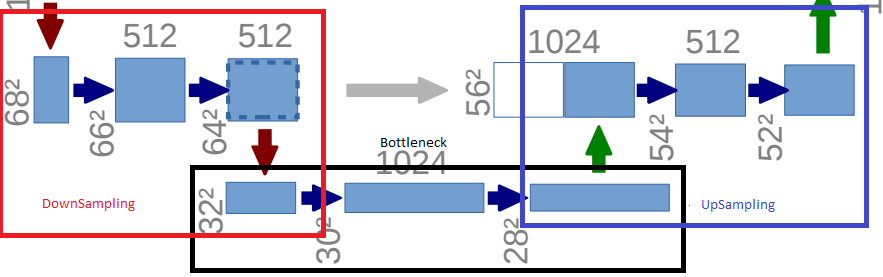
\includegraphics[width=0.5\textwidth]{latex/bottle.png}
    \caption{Bottleneck Block}
    \label{fig:bottleneck}
\end{figure}

The bottleneck block is also \texttt{DoubleConvolution}, without maxpooling. This stage learns the most abstract features before upsampling begins.








\section{Expansive Path (Upsampling)}

\begin{figure}[H]
    \centering
    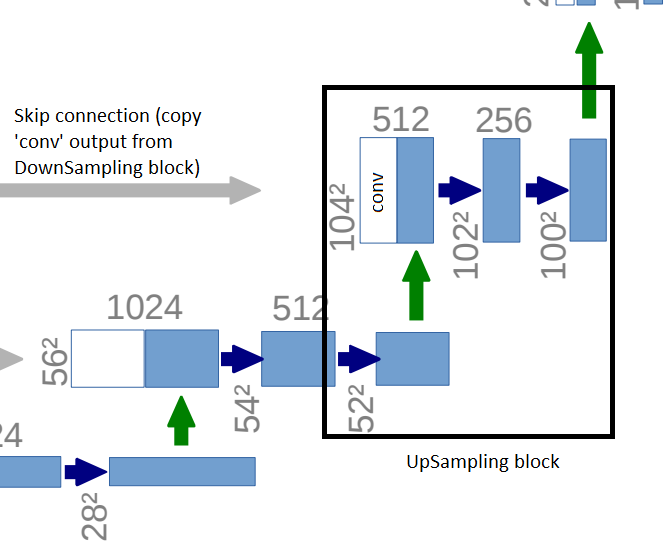
\includegraphics[width=0.5\textwidth]{latex/upsampling2.png}
    \caption{UpSampling Block}
    \label{fig:upsampling}
\end{figure}

The \texttt{UpSampling} block can be implemented as:

\begin{minted}[fontsize=\small, linenos]{python}
class UpSampling(nn.Module):
    def __init__(self, in_channels, out_channels):
        super().__init__()
        self.up = nn.ConvTranspose2d(in_channels, in_channels//2, kernel_size=2, stride=2)
        self.conv = DoubleConvolution(in_channels, out_channels)
    
    def forward(self, x1, x2):
        x1 = self.up(x1)
        x = torch.cat((x1, x2), dim=1)
        return self.conv(x)
\end{minted}

Explanation of the code:

\begin{itemize}
    \item The \texttt{ConvTranspose2d} layer is used for upsampling. Its a $2\times 2$ deconvolution (reverse of regular convolution - it increases spatial resolution).
    \item The output of the \texttt{ConvTranspose2d} layer is concatenated with the corresponding feature map from the contracting path (the skip connection). i.e. this is the output \texttt{conv} of the \texttt{DownSampling} block.
    \item Finally, \texttt{DoubleConvolution}
\end{itemize}








\section{U-Net: Skip connections \& Final layer}

The skip connections are implemented by concatenating the feature maps from the contracting path with the corresponding feature maps in the expansive path. This allows the network to retain spatial information lost during downsampling. It is not \texttt{ResidualBlock} connections, where we add the feature maps: instead we concat them.

Here is the final U-Net coming together:

\begin{minted}[fontsize=\small, linenos]{python}
class UNet(nn.Module):
    def __init__(self, in_channels, num_classes):
        super().__init__()
        self.dconv1 = DownSampling(in_channels, 64)
        self.dconv2 = DownSampling(64, 128)
        self.dconv3 = DownSampling(128, 256)
        self.dconv4 = DownSampling(256, 512)

        self.bottle_neck = DoubleConvolution(512, 1024)

        self.uconv1 = UpSampling(1024, 512)
        self.uconv2 = UpSampling(512, 256)
        self.uconv3 = UpSampling(256, 128)
        self.uconv4 = UpSampling(128, 64)

        self.out = nn.Conv2d(64, num_classes, kernel_size=1)

    def forward(self, x):
        d1,p1 = self.dconv1(x)
        d2,p2 = self.dconv2(p1)
        d3,p3 = self.dconv3(p2)
        d4,p4 = self.dconv4(p3)

        b = self.bottle_neck(p4)
        
        u1 = self.uconv1(b, d4)
        u2 = self.uconv2(u1, d3)
        u3 = self.uconv3(u2, d2)
        u4 = self.uconv4(u3, d1)

        out = self.out(u4)
        return out
\end{minted}

Explanation of the code:

\begin{itemize}
    \item Line 16: the final output layer is a $1 \times 1$ convolution that reduces the number of feature maps to the number of classes in the segmentation task.
    \item Line 19-22: the downsampling blocks. We get dX and pX where dX is the output of the \texttt{DoubleConvolution} block and pX is the output of the maxpooling operation. The pX is used for the next downsampling block and dX is used for the skip connection (lines 26-29).
    \item Line 24: the bottleneck block.
    \item Line 26-29: the upsampling blocks. We get uX which is the output of the \texttt{UpSampling} block. The input is the dX which we talked about before (the skip connection), and the output is the uX which is used for the next upsampling block.
    \item Line 31: the final output layer. The output is the number of classes in the segmentation task.
\end{itemize}



\end{document}